% This is samplepaper.tex, a sample chapter demonstrating the
% LLNCS macro package for Springer Computer Science proceedings;
% Version 2.20 of 2017/10/04
%
\documentclass[runningheads]{llncs}
%
\usepackage{graphicx}
\usepackage{changepage}
\usepackage{cite}
% Used for displaying a sample figure. If possible, figure files should
% be included in EPS format.
%
% If you use the hyperref package, please uncomment the following line
% to display URLs in blue roman font according to Springer's eBook style:
% \renewcommand\UrlFont{\color{blue}\rmfamily}

\begin{document}
%
\title{A decomposition based on constrained clustering algorithms for job shop scheduling problems\thanks{Supported by organization x.}}
%
%\titlerunning{Abbreviated paper title}
% If the paper title is too long for the running head, you can set
% an abbreviated paper title here
%
\author{Mohammed M. S. El-Kholany\inst{1}\orcidID{0000-1111-2222-3333} \and
Second Author\inst{1}\orcidID{1111-2222-3333-4444} \and
Third Author\inst{1,2}\orcidID{2222--3333-4444-5555}}
%
\authorrunning{M. El-Kholany et al.}
% First names are abbreviated in the running head.
% If there are more than two authors, 'et al.' is used.
%
\institute{Alpen-Adria-Universität Klagenfurt, Klagenfurt, Austria 
\email{\{mohammed.el-kholany, konstantin.schekotihin and martin.gebser\}@aau.at}\\
%\url{http://www.springer.com/gp/computer-science/lncs} \and
Technische Universität Graz, Graz, Austria\\
\email{mgebser@ist.tugraz.at}}
%
\maketitle              % typeset the header of the contribution
%
\begin{abstract}
Scheduling decision in production planning plays a significant role in the manufacturing industry. A good schedule may lead to solve production problems and improve productivity. Job-shop Scheduling Problem (JSP) is one of the most crucial problems in production systems. JSP deals with allocating tasks on resources and determining the sequence of the operations on each machine. The main objective of JSP is to complete the processing of all operations in a minimal time. One of the most effective approaches studied by many researchers for solving the JSP is decomposition. This work aims to apply the decomposition strategy to split the problem into a series of sub-problems using data mining methodologies. We will propose a clustering algorithm to group the data points (operations) into clusters, where each cluster is a Time Window. The decomposition process depends on two main phases; the first phase is to extract features to predict the sequence of the operations on each machine. These features are extracted either from the problem itself or from solutions obtained by other heuristics. The second phase is to develop a constrained clustering algorithm to assign each data object (an operation) into a cluster. We solved the problem using the Answer Set Programming model, and we tested our proposed algorithm on a set of benchmark instances, and the results showed that our proposed outperformed other heuristics in most cases. The results also showed that some features like \textit{Remaining Processing Time}, \textit{Machine Load} and \textit{Earliest starting Time} have a significant impact on the solution quality.

\keywords{Job-shop Scheduling  Problem \and Constrained Clustering \and Time Windows \and Answer Set Programming.}
\end{abstract}
%
%
%
\section{Introduction}
Nowadays, the massive progress and development of the internet and online technologies, data generated by machines and devices, product development, quality and inventory management systems, or production planning systems has become huge and is expected to increase in the coming years. Hence, to capture long-term revenues and sustainable competitive advantages, companies must manage the knowledge and have the valuable information to make the right decision at the right time \cite{benabdellah2019survey}. \\

It can be assumed that knowledge management is a crucial issue in the industry. To extract implicit, unknown, and potentially useful information from data, we use data mining techniques that have been responsible for many of artificial intelligence’s recent successes. 
Clustering is one of these techniques, which is applied whenever the extracted data is not labeled, i.e., the semantics of this data is with respect to the application is unclear. Therefore, clustering has always been an exploratory but critical task in the knowledge discovery process, with applications ranging from image processing, production systems, and information retrieval \cite{benabdellah2019survey}. Clustering is a technique that aims to partition a dataset (objects) into subsets by identifying similar objects and aggregating them in the same cluster while the dissimilar objects should belong to different clusters.\\

The data sets could be composed entirely of either numeric features or symbolic features. For the numeric feature, we will use the Euclidean distance metric. However, for symbolic features, the Hamming distance is computed. Since our problem contains only numeric features, we will use Euclidean distance to determine the distance between the objects \cite{aloise2009np, wagstaff2001constrained,macqueen1967some}.\\
%\comment{The next paragraph jumps to a distance, which is one of the similarity measures in the Euclidean space. One should explain this transition.}

Furthermore, from an optimization perspective, the main objective is to minimize the distance between objects falling in the same cluster and maximize the distance between the others that belong to different clusters. Since clustering does not use a subset of the dataset as labels to learn a classification model, clustering differs from classification \cite{wagstaff2001constrained}. In other words, with the terminology of machine learning, clustering is a form of an unsupervised task, which calculates the similarity between data objects without knowing the proper attribution~\cite{li2018geometric}. Due to these unsupervised characteristics, clustering is known as one of the most challenging machine learning tasks \cite{benabdellah2019survey}. \\

Clustering has been widely applied in several disciplines; one is production-planning systems~\cite{nananukul2013clustering,koskosidis1992clustering}, more specifically scheduling \cite{yashar2013multi,tong2016research}. 
%\comment{Are there any citations for the claim above?}
Scheduling is one of the most complex problems in the industry. Scheduling of operations involves resource allocation over a period of time to perform a series of tasks, where one of the most critical problems is the Job-shop Scheduling Problem (JSP). The JSP has been known as a complex and combinatorial optimization problem, and it has been proven to be NP-hard \cite{baker1974introduction,lenstra1979computational}. Therefore, it is very difficult to reach an optimal solution in a reasonable time, even for small instances. However, from a practical perspective, the JSP scale is large, where the number of operations can be up to 10,000s in some workshops \cite{zhang2010hybrid}.


\section{Literature Review}

In this section, we will review some of the most related works about data mining approaches employed to solve scheduling problems. Over the last decades, solving the scheduling problem has attracted the interest of many researchers, and a wide range of approaches has been developed for solving the scheduling problem. One of the approaches that have been widely used to solve the problem is data mining. The main idea of data mining is to explore the patterns from the obtained solutions by some heuristics and then develop some decision rules that approximate the order of the operations in each machine \cite{ismail2012production}. More precisely, it aims to get an order of the operations according to some characteristics.\\

Data mining methodologies are applied to explore the patterns in data generated by Genetic Algorithm (GA) \cite{koonce2000using}. This work aimed to generate rules to determine the priority for each job with weight. They solved the scheduling problem using GA to create some rules. Some characteristics (rank of operations, processing time, machine load, and remaining processing time) have been considered. In order to evaluate their heuristic, they tested the generated rules on some other instances that were randomly generated. The results showed that the generated rules were able to outperform the shortest processing time heuristic. One of the drawbacks is that the problem instances considered contain only 36 operations.\\

Other researchers also implemented GA to get some information of the solution but considered other features to generate decision rules \cite{harrath2002genetic}. They considered processing time, job length, remaining processing time, the rank of the operation, and machine load. To build a generic model for scheduling problems, they discretized the data by converting the quantitative data into qualitative. They sorted the operations share the same machine according to processing time. If two or more operations have the same processing time, they look at the time length of the job. If the job length is the same, sort them out based on the remaining processing time.\\

The work mentioned above had considered static JSP. However, dynamic JSP became one of the most crucial problems in real-life applications. New dispatching rules for JSP are presented using a data mining approach to obtain an efficient schedule in a dynamic Job-shop Scheduling environment \cite{shahzad2010discovering}. This study aimed to minimize makespan by creating new dispatching rules. Firstly, they solved the scheduling problems using Tabu Search and used the obtained solution as a training set to get a rule-set capable of approximating efficient solutions. They considered some other features like (Earliest possible Starting Time EST, the difference in remaining processing time for a job, and the difference in the processing time of two operations) to create a rule-set for dispatching the operations. The experiments showed that the results of mined rule-set are superior or comparable to the heuristics in the literature.\\

The variable neighborhood search (VNS) is combined with the k-means algorithm to address Dynamic JSP \cite{adibi2014clustering}. The proposed algorithm depends on extracting information from the problem's input data when an event like (machine breakdown or adding new job(s)) occurred. At any rescheduling point, cluster analysis is performed to replace jobs according to their distances. In other words, a job that belongs to a farther cluster has a greater probability to be selected in making a new adjacent than the other belonging to a closer cluster. The proposed method was compared to VNS and some common heuristics using a simulated job shop. the results indicated that the performance of the proposed model is better than the others, including some heuristics (FIFO, LIFO, and SPT).\\

Another study has presented a data mining approach to generate an initial population for population-based heuristics/metaheuristics to solve JSP \cite{nasiri2019data}. They extracted information from optimal or near-optimal solutions obtained by a heuristic procedure called "Assignment Procedure" to build decision rules to determine the priority of the operations. Once the rules are extracted, the initial solution is generated using these rules. To evaluate the performance of the proposed method, they performed a series of computational experiments on several test instances. The results showed that the proposed method with data mining generated initial population outperforms the methods with randomly generated initial population.\\

From the literature, we have found that most of the studies which used data mining techniques aimed to extract some features either from the problem instances or solutions obtained by some heuristics to build a decision-rules to order the operations assigned to a machine. Our study aims to  find the most appropriate sequence of operations to optimize the typical performance indicator (makespan). Several approaches have been studied to solve JSP, and one of the most effective approaches used is decomposition \cite{zhang2010hybrid,zhai2014decomposition}. The main idea of the decomposition is to split the problem into a series of sub-problems (windows) and solve each of them separately in a sequence, and then obtain the solution of the original problem.\\

This work intends to apply the clustering techniques to decompose the problem into sub-problems, where the number of clusters corresponds to the number of sub-problems (windows), and the operations correspond to data objects. For the JSP, an instance consists of a set of jobs to be processed on machines. The number of jobs is $n$, and the number of machines is $m$. Each job contains $m$ operations with the operation precedence constraints. Each operation should be executed on machine $m$ for a certain amount of time. Since the problem at hand has precedence constraints, it is required to apply a constrained clustering approach for the decomposition \cite{wagstaff2001constrained}.\\

It can be said that the attributes of the classical JSP are quite a few and not sufficient to define the similarity and dissimilarity between the operations. The lack of these attributes guides us to extract more features that could specify which operations are similar and should be in the same window and which shall not be in the same window. The main contribution of this work is to extract some features that have a significant impact on the decomposition process and accordingly on the makespan. 
More specifically, we need to extract some features to define which operations are similar to be scheduled in the same window and get a near-optimal solution in a reasonable time. \\

This work consists of two main phases:

\begin{enumerate}
    \item The first phase is to apply data mining to predict the order of each operation on its machine according to some features. In this phase, we will try to get all possible features extracted from the problem itself, which significantly affect the quality of the solution. In addition, we will use some heuristics such as (FIFO, MTWR, EST) to learn the pattern of the solutions obtained by those.

    \item The second phase aims to develop, implement and test a proposed clustering algorithm that will split the problem into sub-problems where each operation is a data object, and each cluster will represent a time window. It will consider the precedence constraints between the operations and balancing between the clusters according to the number of operations per cluster.
\end{enumerate}


\section{Features extraction}
In this section, we will show which features have been extracted and how did we extract them. Based on the previous work, \cite{koonce2000using, harrath2002genetic, shahzad2010discovering, ismail2012production, adibi2014clustering, nasiri2019data}, the following features have been identified: priority, processing time, remaining processing time, machine load, and route position. Most of the researchers converted the attributes into qualitative data. As mentioned in these studies, the main reason for this conversion is to make the decision rules more generic, which can be applied to several scheduling problems. However, in our case, we will not convert the data into classes because we will use these features to measure the similarities/dissimilarities between the operations in the clustering process, which requires having numerical values.
We will show the features that we considered:
\subsection{\textit{Process}}
\textit{Processing Time (PT)}  and \textit{Remain Processing Time (RPT)} are attributes dependent on the problem domain. The \textit{PT} represents the execution time of a particular operation in a machine. However, \textit{RPT} is the aggregate processing time for all subsequent operations of that job.

\subsection{\textit{Operation}}
The \textit{Operation} attribute is an ordinal value to represent the rank of each operation in its job.

\subsection{\textit{Time Length of a Job}(TLJ)}
\textit{TLJ} is an attribute that describes the total processing time needed to complete a particular job. It is the summation of processing time for all operations of that job.

\subsection{\textit{Earliest Starting Time} (EST)}
The \textit{EST} attribute represents the earliest possible time for a particular operation to be executed. It is calculated by accumulating the processing time of the predecessor(s) of that operation, and it is $Zero$, if the operation has no predecessor.

\subsection{\textit{Machine Load} (ML)}
\textit{ML} is a property of a machine that shows how much time a particular machine has to execute all the operations assigned to it. In the initial state, the \textit{ML} is the aggregate of processing time of all operations assigned to that machine. For each step, the load of a machine is decreased by the processing time of an operation assigned to the machine and has the smallest \textit{EST}.

\subsection{\textit{Starting Time} (ST)}
\textit{ST} attribute represents the starting execution time of each operation by solving the problem using heuristics FIFO, MTWR and EST developed by \cite{tassel2021reinforcement,el2020job}.

\subsection{\textit{Waiting Time} (WT)}
Since we used three different heuristics to mine information from the obtained solution, we will have three waiting times. \textit{WT} attribute is the difference between the starting time of a particular operation and the maximum value between the end time of its predecessor and when the machine became free.

\section{Proposed Algorithm}

In this section, we will show the implementation of our proposed model and how it works. The main idea of the proposed model is to split the problem into sub-problems, solve them sequentially and integrate the solutions to have the solution of the main problem. We aim to decompose the problem into time windows because this technique proved its effectiveness for solving the scheduling problems. Several ways have been presented during the last decades to decompose the problem  \cite{zhai2014decomposition,singer2001decomposition,ovacik2012decomposition,uzsoy2000performance}.\\ 

The proposed model aims to apply clustering methods where each cluster will represent a time window, and each operation is a data object. The clustering algorithms are used to group a set of data objects into one cluster. It depends on measuring the similarity/dissimilarity between the data objects according to the features of these data objects. The similar objects will be in one cluster, and the dissimilar are in different clusters. The difference between the basic clustering and our proposed is the ordering of the clusters. In general, the cluster number does not have meaning; it just means that the data objects grouped in a particular cluster are similar. However, in our case, the cluster number is meaningful because the data objects grouped in cluster $i$ should be scheduled before other data objects in cluster $i+1$. More specifically, it is not allowed to insert a data object (\textit{an operation}) in a particular cluster, and the predecessor of that operation is not assigned yet to the same cluster or the preceding cluster(s). Since we will solve each window separately, we should consider balancing the clusters concerning the number of operations assigned to each cluster. So that, we will have two types of constraints:
\begin{enumerate}
\item The predecessor(s) of an operation must be inserted into the same or previous cluster(s).
\item The number of operations assigned to each cluster should be close to each other.
\end{enumerate}

Fig.~\ref{fig1} shows a flowchart of the proposed algorithm. As shown in the flowchart, the number of clusters is given. We calculate the cluster capacity by dividing the total number of operations by the number of clusters. In the next step, the clustering process started by generating the centroids, where the number of centroids is the number of clusters. In general, the centroids are generated randomly as well as in our model. However, we selected some operations as centroids. Although the operations are selected randomly, we followed a rule to select the centroids. For example, let us assume that a job consists of 15 operations, and three centroids should be generated. The first centroid will be an operation of rank 1 - 5, the second centroid will be 6 - 10, and the third will be from the last five operations. We followed this strategy to make them far from each other because the operations grouped in the first clusters should be at the beginning of their jobs. After generating the centroids, we perform a double-check for exceeding the number of clusters and the cluster capacity, respectively. After that, we calculate the distance between each operation and the centroid of the current cluster using Euclidean distance and assign the nearest operation to that cluster. In order to satisfy the precedence constraint, we check if the predecessor is not assigned to a cluster, it will be assigned to the current cluster, and the centroid is updated. If the maximum number of operations is reached, we will go to the next cluster. After assigning all operations into clusters, the algorithm terminates.

\begin{figure}[h!]
  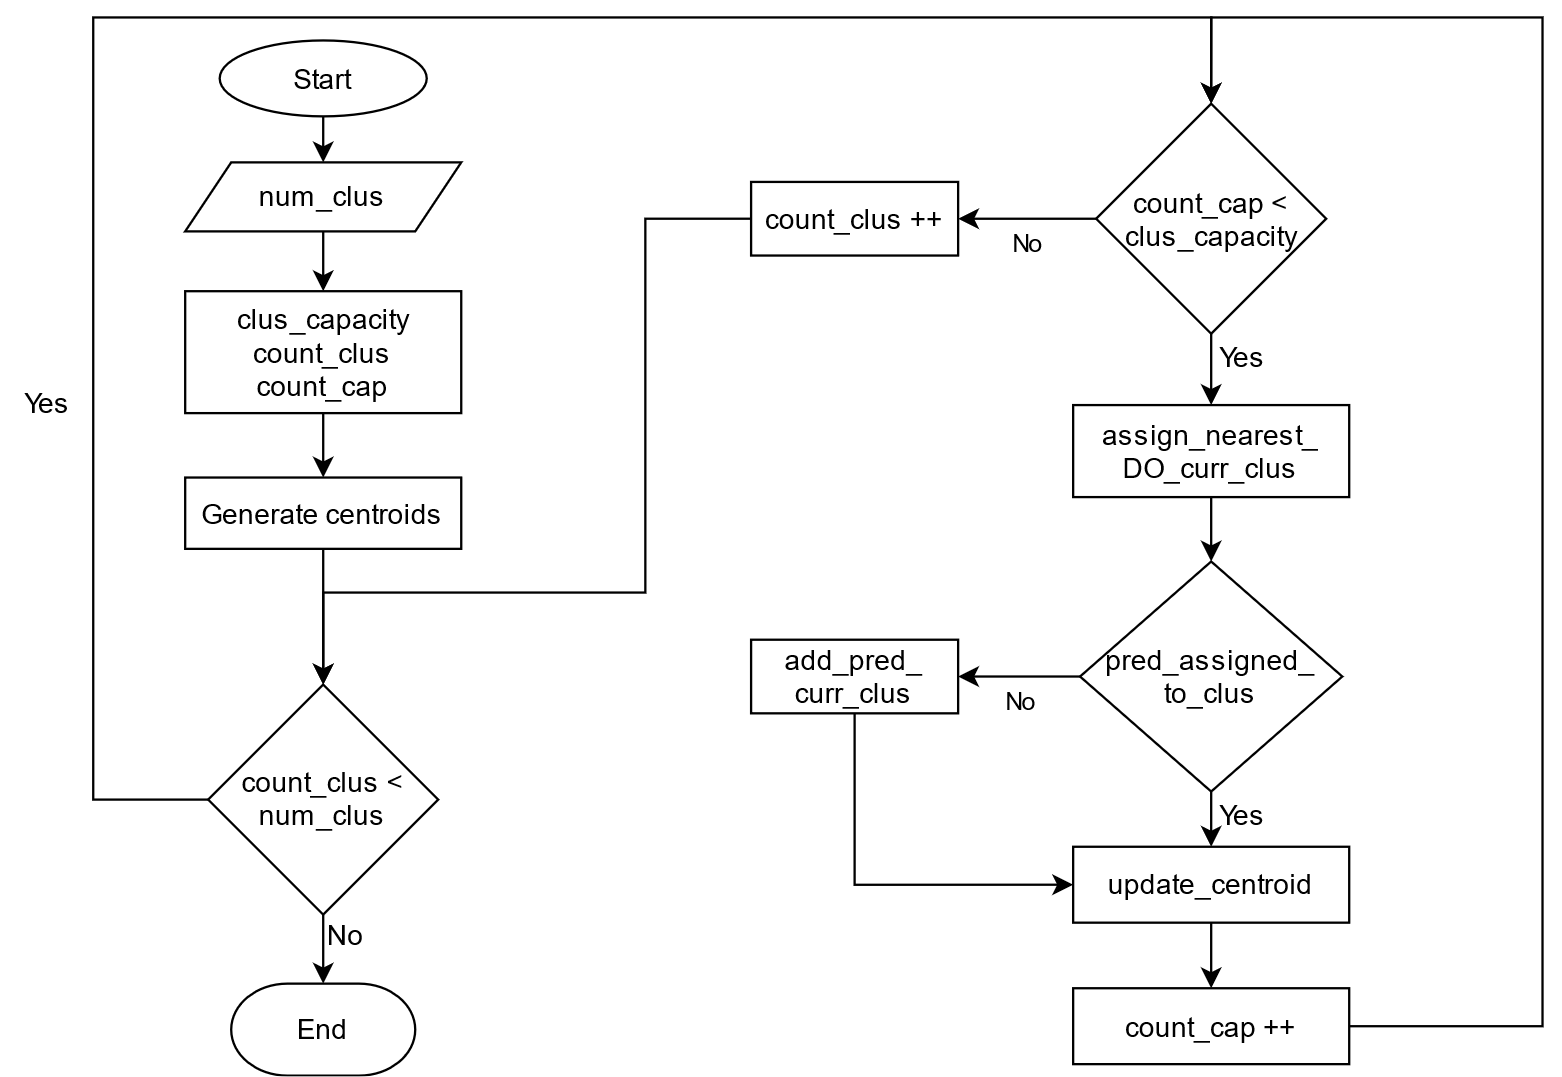
\includegraphics[width=\linewidth]{Flow_chart_9.png}
  \caption{Flowchart of the proposed Clustering Algorithm.}
  \label{fig1}
\end{figure}

\section{Results}
We use the benchmark instances presented in \cite{taillard1993benchmarks} as a dataset to work on. Many researchers have studied these instances and presented different approaches to solving them. We also developed different decomposition strategies to solve those. Therefore, it will be possible to measure the success/failure of our proposed model by comparing the results of the strategies developed in the past with those obtained from the proposed algorithm. There are 12 features, as we described in the previous section. In order to know which features have a significant effect on the results, we did some combinations of the features to perform the decomposition process clustering-based and then solved the problem using the Answer Set Programming model developed in \cite{el2020job} with a timeout of 10 minutes. The combinations of the selected features are listed as follows:
\begin{enumerate}
\item \textbf{F1} \textrightarrow \textit{\{ ST\textunderscore FIFO, ST\textunderscore MTWR, ST\textunderscore EST \}}
\item \textbf{F2} \textrightarrow \textit{\{ ST\textunderscore FIFO, ST\textunderscore MTWR, ST\textunderscore EST, RPT \}} 
\item \textbf{F3} \textrightarrow \textit{\{ ST\textunderscore FIFO, ST\textunderscore MTWR, ST\textunderscore EST, EST \}} 
\item \textbf{F4} \textrightarrow \textit{\{ ST\textunderscore FIFO, ST\textunderscore MTWR, ST\textunderscore EST, ML \}} 
\item \textbf{F5} \textrightarrow \textit{\{ ST\textunderscore FIFO, ST\textunderscore MTWR, ST\textunderscore EST, RPT, EST \}}
\item \textbf{F6} \textrightarrow \textit{\{ ST\textunderscore FIFO, ST\textunderscore MTWR, ST\textunderscore EST, RPT, ML \}} 
\item \textbf{F7} \textrightarrow \textit{\{ ST\textunderscore FIFO, ST\textunderscore MTWR, ST\textunderscore EST, EST, ML \}} 
\item \textbf{F8} \textrightarrow \textit{\{ ST\textunderscore FIFO, ST\textunderscore MTWR, ST\textunderscore EST, WT\textunderscore FIFO, WT\textunderscore MTWR, WT\textunderscore EST \}} 
\item \textbf{F9} \textrightarrow \textit{\{ ST\textunderscore FIFO, ST\textunderscore MTWR, ST\textunderscore EST, WT\textunderscore FIFO, WT\textunderscore MTWR, WT\textunderscore EST, RPT \}} 
\item \textbf{F10} \textrightarrow \textit{\{ ST\textunderscore FIFO, ST\textunderscore MTWR, ST\textunderscore EST, WT\textunderscore FIFO, WT\textunderscore MTWR, WT\textunderscore EST, EST \}} 
\item \textbf{F11} \textrightarrow \textit{\{ ST\textunderscore FIFO, ST\textunderscore MTWR, ST\textunderscore EST, WT\textunderscore FIFO, WT\textunderscore MTWR, WT\textunderscore EST, ML \}}
\item \textbf{F12} \textrightarrow \textit{\{ ST\textunderscore FIFO, ST\textunderscore MTWR, ST\textunderscore EST, WT\textunderscore FIFO, WT\textunderscore MTWR, WT\textunderscore EST, RPT, EST \}}
\item \textbf{F13} \textrightarrow \textit{\{ ST\textunderscore FIFO, ST\textunderscore MTWR, ST\textunderscore EST, WT\textunderscore FIFO, WT\textunderscore MTWR, WT\textunderscore EST, RPT, ML \}}
\item \textbf{F14} \textrightarrow \textit{\{ ST\textunderscore FIFO, ST\textunderscore MTWR, ST\textunderscore EST, WT\textunderscore FIFO, WT\textunderscore MTWR, WT\textunderscore EST, EST, ML \}}
\item \textbf{F15} \textrightarrow \textit{\{ ST\textunderscore FIFO, ST\textunderscore MTWR, ST\textunderscore EST, WT\textunderscore FIFO, WT\textunderscore MTWR, WT\textunderscore EST, RPT, EST, ML \}}
\end{enumerate}
We neglected the rank of an operation and the time length of a job because they had negative impact results from the preliminary experiments. The following Table~\ref{tab1} shows the selected features, and the performance of each combination for solving benchmark instances of 50 jobs and 15 machines \cite{taillard1993benchmarks}. The following table shows the results of our experiments. The first column represents the instances we tested, and the next three columns show the makespan values obtained by FIFO, MTWR, and EST heuristics. From the fifth column, we show the makespan values obtained by combining the features mentioned above. Our experiments found that the first five combinations do not provide good solutions compared to the other heuristics. However, features (\textbf{F6}, \textbf{F8}, \textbf{F11}, \textbf{F12}, \textbf{F14} and \textbf{F15}) have a good impact in the cost function in the most cases. Especially, combinations \textbf{F6} and \textbf{F15} provided good results. It means that the most important features extracted from the problem itself and have a positive impact on the performance are \textit{Remaining Processing Time, Machine Load and Earliest Starting Time}. Also, The information obtained from the solutions of the other heuristics like (\textit{Starting Time} and \textit{Waiting Time}) led us to get better decomposition for the problem at hand. More specifically, combining \textit{Remaining Processing Time} with \textit{Machine Load} provides a good decomposition with/without \textit{Waiting Time} attributes obtained by the other heuristics.
\begin{table}[h!]
\setlength{\tabcolsep}{4.0pt}
  \begin{center}
    \caption{The performance of selected features.}
    \label{tab1}
 \begin{adjustwidth}{-3.7cm}{}
    \begin{tabular}{c|c|c|c|c|c|c|c|c|c|c|c|c|c|c|c|c|c|c|c}
      \textbf{Instances} & \textbf{FIFO} & \textbf{MTWR} & \textbf{EST} & \textbf{F1} & \textbf{F2} & \textbf{F3} & \textbf{F4} & \textbf{F5} & \textbf{F6} & \textbf{F7} & \textbf{F8} & \textbf{F9} & \textbf{F10} & \textbf{F11} & \textbf{F12} & \textbf{F13} & \textbf{F14} & \textbf{F15}\\
      \hline
      TA51 &3549  &3364  &3833  &3506  &3362  &3324  &3360  &3346  &\textbf{3294}  &3328  &3588  &3588  &3568  &3514  &3682  &3624  &3554  &3509 \\
      TA52 &3339  &3304  &3594  &3277  &3318  &3330  &3286  &3243  &3275  &3226  &3397  &3373  &3533  &3256  &3494  &3505  &3373  &\textbf{3184} \\
      TA53 &3160  &3168  &3443  &3382  &3585  &3347  &3543  &3517  &3250  &3338  &3251  &3522  &3373  &3585  &\textbf{3143}  &3427  &3524  &3380 \\
      TA54 &3218  &3494  &3439  &3414  &3425  &3425  &3503  &3397  &3265  &3353  &3563  &3443  &3386  &3352  &3270  &3236  &3232  &3289 \\
      TA55 &3291  &3237  &3784  &3308  &3441  &3424  &3319  &3355  &3386  &3301  &3498  &3385  &3530  &3365  &3309  &3370  &3385  &\textbf{3218} \\
      TA56 &3325  &3287  &3552  &3353  &3380  &3548  &3270  &3383  &3366  &3564  &\textbf{3229}  &3306  &3362  &3344  &3332  &3338  &3483  &3389 \\
      TA57 &3654  &3633  &3681  &3605  &3573  &3601  &3583  &3650  &\textbf{3480}  &3592  &3621  &3543  &3608  &3670  &3632  &3749  &3573  &\textbf{3480} \\
      TA58 &3299  &3591  &3764  &3352  &3412  &3370  &3509  &3707  &\textbf{3324}  &3496  &3517 &3716 &3644  &3611  &3471  &3437  &3365   &3481 \\
      TA59 &3344  &3394  &3661  &3453  &3416  &3301  &3339  &3508  &3430  &3352  &3258 &3381  &3402  &\textbf{3145}  &3250  &3253  &3284  &3290 \\
      TA60 &3129  &3257  &3399  &3483  &\textbf{3315}  &3617  &3563  &3591  &3327  &3399  &3374  &3526  &3637  &3425  &3676  &3659  &3767  &3569 \\
    \end{tabular}
\end{adjustwidth}
  \end{center}
 
\end{table}


\section{Conclusion}
Data mining and machine learning is an area of interest in many manufacturing companies and other fields. In order to increase productivity and decrease the operation cost, there should be high-quality schedules to be used. This study focused on data mining and clustering approaches for solving the Job-shop Scheduling Problem. The first issue in this work is to explore the knowledge in good schedules and try to use this knowledge to get more efficient schedules. We extracted some features from the problem at hand and other features from schedules obtained by heuristics. The second issue is finding a powerful way to decompose the problem into windows where each cluster is a window and solve them sequentially. In order to split the problem, we proposed a constrained clustering algorithm considering the precedence constraints of the JSP. We tested our model on benchmark instances, and the results showed that the performance of the proposed model outperforms other heuristics FIFO, MTWR, and EST; and some attributes like (\textit{Starting Time, Waiting Time, Remaining Processing Time, and Machine Load}) played an important role to split the operations in a good way. There are several ways to extend this study. Firstly, solve bigger instances and others in a real-life application in which more features could be extracted. Secondly, develop other clustering algorithms to split the problem more efficiently and get better results.

\bibliographystyle{splncs04}
\bibliography{references}


\end{document}
